\documentclass[notes,11pt, aspectratio=169]{beamer}

\usepackage{pgfpages}
% These slides also contain speaker notes. You can print just the slides,
% just the notes, or both, depending on the setting below. Comment out the want
% you want.
\setbeameroption{hide notes} % Only slide
%\setbeameroption{show only notes} % Only notes
%\setbeameroption{show notes on second screen=right} % Both

\usepackage{helvet}
\usepackage[default]{lato}
\usepackage{array}
\usepackage{tgbonum}

\usepackage{tikz}
\usepackage{verbatim}
\setbeamertemplate{note page}{\pagecolor{yellow!5}\insertnote}
\usetikzlibrary{positioning}
\usetikzlibrary{snakes}
\usetikzlibrary{calc}
\usetikzlibrary{arrows}
\usetikzlibrary{decorations.markings}
\usetikzlibrary{shapes.misc}
\usetikzlibrary{matrix,shapes,arrows,fit,tikzmark}
\usepackage{amsmath}
\usepackage{mathpazo}
\usepackage{hyperref}
\usepackage{lipsum}
\usepackage{multimedia}
\usepackage{graphicx}
\usepackage{multirow}
\usepackage{graphicx}
\usepackage{dcolumn}
\usepackage{bbm}
\newcolumntype{d}[0]{D{.}{.}{5}}

\usepackage{changepage}
\usepackage{appendixnumberbeamer}
\newcommand{\beginbackup}{
   \newcounter{framenumbervorappendix}
   \setcounter{framenumbervorappendix}{\value{framenumber}}
   \setbeamertemplate{footline}
   {
     \leavevmode%
     \hline
     box{%
       \begin{beamercolorbox}[wd=\paperwidth,ht=2.25ex,dp=1ex,right]{footlinecolor}%
%         \insertframenumber  \hspace*{2ex} 
       \end{beamercolorbox}}%
     \vskip0pt%
   }
 }
\newcommand{\backupend}{
   \addtocounter{framenumbervorappendix}{-\value{framenumber}}
   \addtocounter{framenumber}{\value{framenumbervorappendix}} 
}


\usepackage{graphicx}
\usepackage[space]{grffile}
\usepackage{booktabs}
\newcommand\independent{\protect\mathpalette{\protect\independenT}{\perp}}
\def\independenT#1#2{\mathrel{\rlap{$#1#2$}\mkern2mu{#1#2}}}
\DeclareMathOperator{\Supp}{Supp}

% These are my colors -- there are many like them, but these ones are mine.
\definecolor{blue}{RGB}{0,114,178}
\definecolor{red}{RGB}{213,94,0}
\definecolor{yellow}{RGB}{240,228,66}
\definecolor{green}{RGB}{0,158,115}

\hypersetup{
  colorlinks=false,
  linkbordercolor = {white},
  linkcolor = {blue}
}


%% I use a beige off white for my background
\definecolor{MyBackground}{RGB}{255,253,218}

%% Uncomment this if you want to change the background color to something else
%\setbeamercolor{background canvas}{bg=MyBackground}

%% Change the bg color to adjust your transition slide background color!
\newenvironment{transitionframe}{
  \setbeamercolor{background canvas}{bg=yellow}
  \begin{frame}}{
    \end{frame}
}

\setbeamercolor{frametitle}{fg=blue}
\setbeamercolor{title}{fg=black}
\setbeamertemplate{footline}[frame number]
\setbeamertemplate{navigation symbols}{} 
\setbeamertemplate{itemize items}{-}
\setbeamercolor{itemize item}{fg=blue}
\setbeamercolor{itemize subitem}{fg=blue}
\setbeamercolor{enumerate item}{fg=blue}
\setbeamercolor{enumerate subitem}{fg=blue}
\setbeamercolor{button}{bg=MyBackground,fg=blue,}



% If you like road maps, rather than having clutter at the top, have a roadmap show up at the end of each section 
% (and after your introduction)
% Uncomment this is if you want the roadmap!
% \AtBeginSection[]
% {
%    \begin{frame}
%        \frametitle{Roadmap of Talk}
%        \tableofcontents[currentsection]
%    \end{frame}
% }
\setbeamercolor{section in toc}{fg=blue}
\setbeamercolor{subsection in toc}{fg=red}
\setbeamersize{text margin left=1em,text margin right=1em} 

\newenvironment{wideitemize}{\itemize\addtolength{\itemsep}{10pt}}{\enditemize}

\usepackage{environ}
\NewEnviron{videoframe}[1]{
  \begin{frame}
    \vspace{-8pt}
    \begin{columns}[onlytextwidth, T] % align columns
      \begin{column}{.70\textwidth}
        \begin{minipage}[t][\textheight][t]
          {\dimexpr\textwidth}
          \vspace{8pt}
          \hspace{4pt} {\Large \sc \textcolor{blue}{#1}}
          \vspace{8pt}
          
          \BODY
        \end{minipage}
      \end{column}%
      \hfill%
      \begin{column}{.38\textwidth}
        \colorbox{green!20}{\begin{minipage}[t][1.2\textheight][t]
            {\dimexpr\textwidth}
            Face goes here
          \end{minipage}}
      \end{column}%
    \end{columns}
  \end{frame}
}

\title[]{\textcolor{blue}{Likelihood Methods: Binary Discrete Choice, GLM and Computational Methods}}
\author[PGP]{}
\institute[FRBNY]{\small{Paul Goldsmith-Pinkham}}
\date{\today}


\begin{document}

%%% TIKZ STUFF
\tikzset{   
        every picture/.style={remember picture,baseline},
        every node/.style={anchor=base,align=center,outer sep=1.5pt},
        every path/.style={thick},
        }
\newcommand\marktopleft[1]{%
    \tikz[overlay,remember picture] 
        \node (marker-#1-a) at (-.3em,.3em) {};%
}
\newcommand\markbottomright[2]{%
    \tikz[overlay,remember picture] 
        \node (marker-#1-b) at (0em,0em) {};%
}
\tikzstyle{every picture}+=[remember picture] 
\tikzstyle{mybox} =[draw=black, very thick, rectangle, inner sep=10pt, inner ysep=20pt]
\tikzstyle{fancytitle} =[draw=black,fill=red, text=white]
%%%% END TIKZ STUFF

% Title Slide
\begin{frame}
\maketitle

\end{frame}


\begin{frame}{Today's topic: minimizing objection functions and an application }
  \begin{columns}[T] % align columns
    \begin{column}{.6\textwidth}
      \begin{wideitemize}
      \item Today: Two topics
        \begin{enumerate}
        \item Minimizing objective functions instead of minimizing squares
        \item Studying binary choice model
        \end{enumerate}
      \item Minimizing objective functions: examples include
        minimizing squared distances, or maximizing likelihoods
      \item Most estimation issues can be framed as general
        objective function minimization problems
      \item Highlight this with example non-linear problems
        \begin{itemize}
        \item Generalized linear models 
        \end{itemize}
      \end{wideitemize}
    \end{column}%
  \hfill%
  \begin{column}{.4\textwidth}
    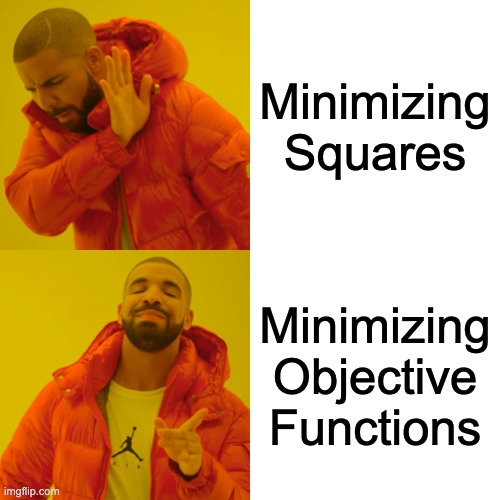
\includegraphics[width=\linewidth]{images/drake_minimization.jpg}
  \end{column}
\end{columns}
\end{frame}



\begin{frame}{Our setup}
  \begin{wideitemize}
  \item Consider the following binary outcome problem: let $Y_{i}$ denote if
    person $i$ is a homeowner, and $X_{i}$ includes three covariates:
    income, age and age$^{2}$ (plus a constant)
  \item A relatively general form of this relationship is 
    $$Y_{i} = F(X_{i},\beta) + \epsilon_{i}$$
    In many ways, no different from our other estimation
    problems with linear regression!
  \item We can talk about an estimand for this setup based on
    assumptions on $F$ and $\epsilon_{i}$
  \end{wideitemize}
\end{frame}

\begin{frame}{Binary model -- what's the right functional form?}
  \begin{wideitemize}
    
  \item We could model this outcome using a linear regression -- why
    not? Assume strong ignorability (or just
    $E(\epsilon_{i} | X_{i}) = 0$) and
    $$E(Y_{i}|X_{i}) = X_{i}\beta \qquad \rightarrow Y_{i} = X_{i}\beta + \epsilon_{i}$$
  \item  The canonical problem with this is twofold:
  \begin{enumerate}
  \item The errors will be unusual -- since it's binary,
    $V(Y|X) = X_{i}\beta (1- X_{i}\beta)$, and you'll have pretty
    significant heteroskedasticity (this is obviously solveable using robust SE)
  \item Except under some special circumstances, it's very likely that
    the predicted values of $Y_{i}$ will be outside of $[0,1]$
  \end{enumerate}
\item What's an example where they will not be? Discrete exhaustive regressors!
  \begin{itemize}
  \item   Why? No extrapolation. Extrapolation is what causes values outside support.
  \end{itemize}
\item How does this impact our causal estimates?
  \begin{itemize}
  \item If the model is correctly specified, we can generate
    counterfactuals
  \item If not, then we get a linear approximation
  \end{itemize}
  \end{wideitemize}
\end{frame}


\begin{frame}{Linear Probability Model estimates on homeownership}
  \begin{columns}[T] % align columns
    \begin{column}{.4\textwidth}
      \begin{wideitemize}
      \item If income were strictly ignorable, we could say that 10k
        increase in income leads to 0.8 p.p. increase in the
        probability of homeownership
      \item Predicted values of homeownership are on support of
        $[0.283, 1.78]$
        \begin{itemize}
        \item Oops.
        \end{itemize}
      \end{wideitemize}
    \end{column}%
  \hfill%
  \begin{column}{.6\textwidth}
    \begin{tabular}{lrr}
      variable &  linear est.  &  std.error\\
      \midrule
      Intercept & 0.0242 &   0.0410\\
      age&   0.0220 &   0.0017\\
      age$^2$&  -0.0002 &   0.0000\\
      income /10k&   0.0069    & 0.0007\\
      \end{tabular}
  \end{column}
\end{columns}
\end{frame}



\begin{frame}{Modeling discrete choice}
  \begin{wideitemize}
    \item  There are two ways to think about how we think about this estimation problem. These
  are not mutually exclusive.
\item The first is a statistical view. E.g. can we model the
  statistical process better (e.g. the counterfactual). One way to
  consider this is $X\beta$ is the conditional mean of some process --
  what is a statistical error term that fits with this?
  \begin{itemize}
  \item Special case of what's termed ``Generalized Linear Models'' (GLM)
  \item Will discuss in a bit
  \end{itemize}
\item   A second way to view this is as an structural (economic) choice
  problem.  Most models of limited dependent variables (e.g. binary)
  instead assume a latent index. 

  $$Y^{*} = X\beta + \epsilon, \qquad Y = 
  \begin{cases}
    1 & Y^{*}>0\\
    0 & Y^{*} \leq 0\\
  \end{cases}
  $$

  \end{wideitemize}

\end{frame}

\begin{frame}{All about the epsilons}
  \begin{columns}[T] % align columns
    \begin{column}{.6\textwidth}
  $$Y^{*} = X\beta + \epsilon, \qquad Y = 
  \begin{cases}
    1 & Y^{*}>0\\
    0 & Y^{*} \leq 0\\
  \end{cases}
  $$
      \begin{wideitemize}
      \item A natural approach is to make a distributional assumption
        about $\epsilon$ to do estimation (and fix the support
        problem). Two common assumptions:
        \begin{enumerate}
        \item $\epsilon$ is conditionally normally distributed (probit), such that
          $Pr(Y_{i} = 1 | X_{i}) = \Phi(X_{i}\beta)$
        \item $\epsilon$ is conditionally extreme value (logistic) such that
          $Pr(Y_{i} = 1 | X_{i}) = \frac{\exp(X_{i}\beta)}{1+\exp(X_{i}\beta)}$
        \end{enumerate}
      \item   Note that these are not, in the binary setting, deeply substantive
        assumptions.
        \begin{itemize}
        \item A challenge for probit models is that there's no closed
          form solution for $\Phi$
        \end{itemize}
      \end{wideitemize}
    \end{column}%
  \hfill%
  \begin{column}{.4\textwidth}
    \begin{center}
      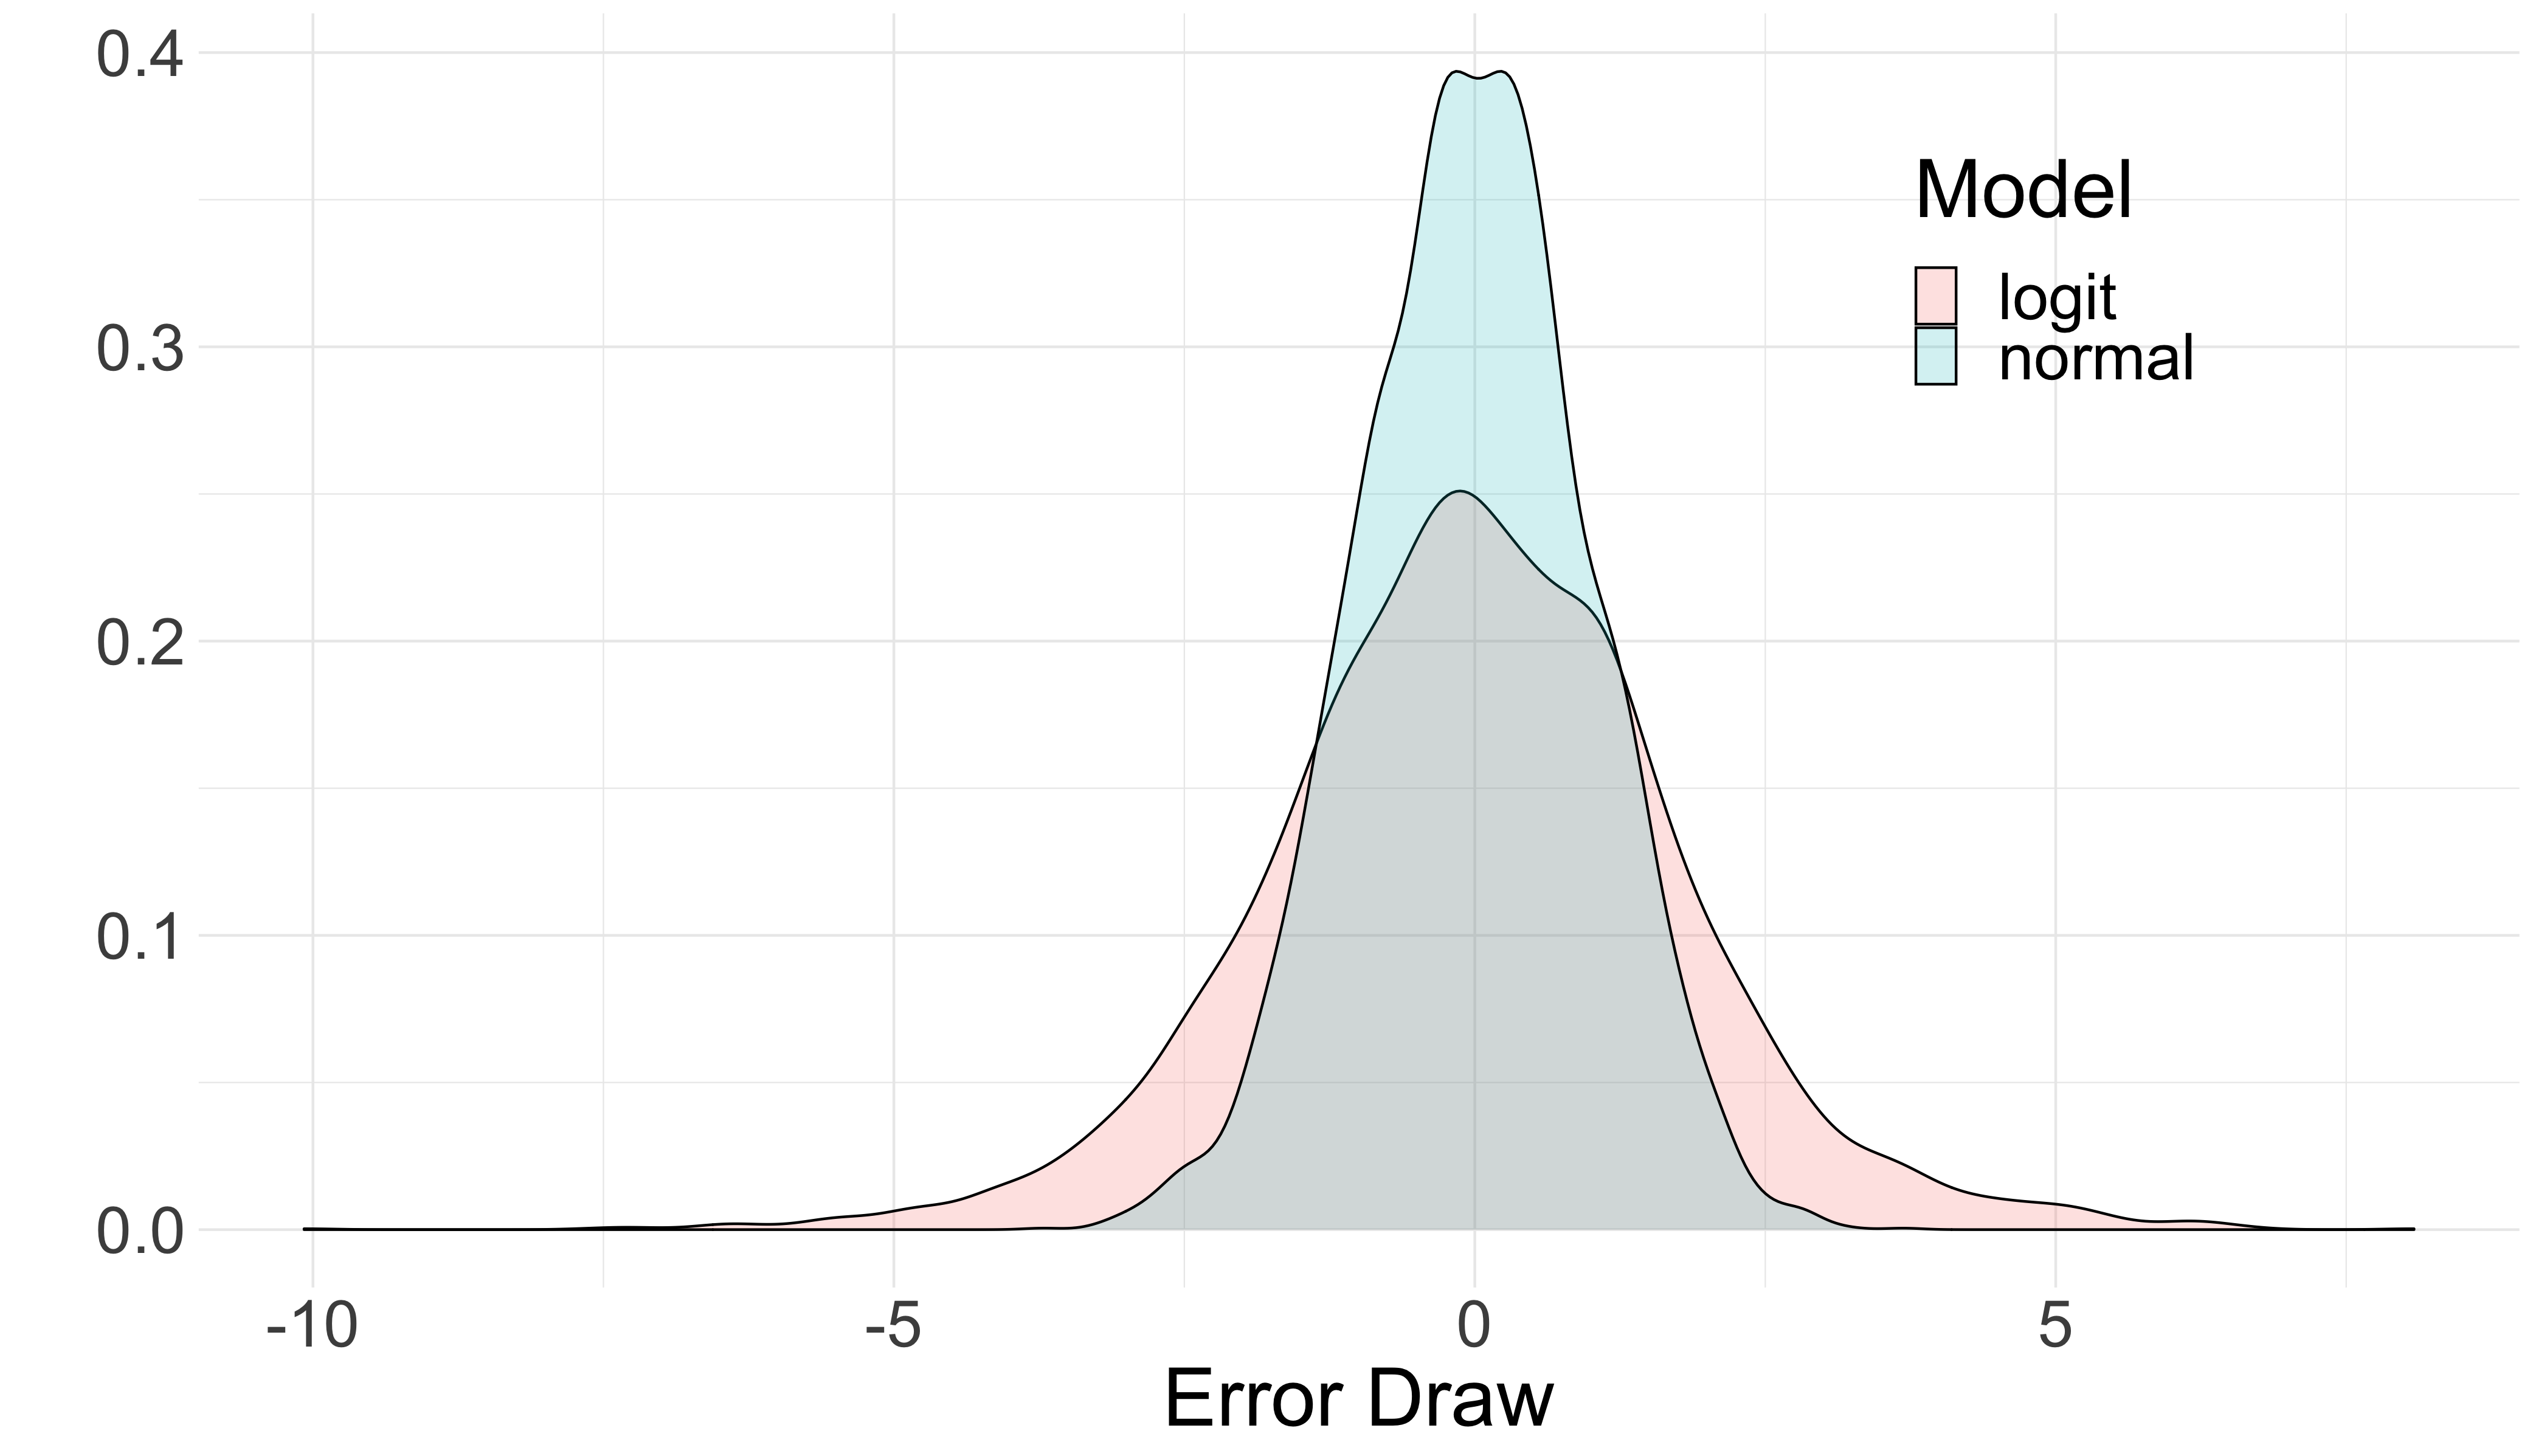
\includegraphics[width=\linewidth]{images/logit_v_normal.png}
    \end{center}
  \end{column}
\end{columns}
  \end{frame}

  \begin{frame}{Identification up to scale}
  \begin{columns}[T] % align columns
    \begin{column}{.6\textwidth}
  $$Y^{*} = X\beta + \epsilon,  \; \Pr(Y_{i} =1|X_{i}) = F(X_{i}\beta)  $$

  \begin{wideitemize}
  \item  Important caveat: these modes only identify $\beta$  up to scale.
  \item   Why?  The ``true'' model of $\epsilon$ could have variance
    $\sigma^{2}$ that is unknown.
  \item Consider if $F(X_{i}\beta) = \Phi(X_{i}\beta)$. If this were a
    general normal (rather than standardized with variance 1), we
    could just scale up the coefficients proportinoate to $\sigma$ and
    the realized binary outcome would identical.  Hence, we normalize
    $\sigma = 1$ in most cases. This is \emph{not} a meaningful
    assumption.
  \end{wideitemize}

    \end{column}%
  \hfill%
  \begin{column}{.4\textwidth}
    \begin{center}
      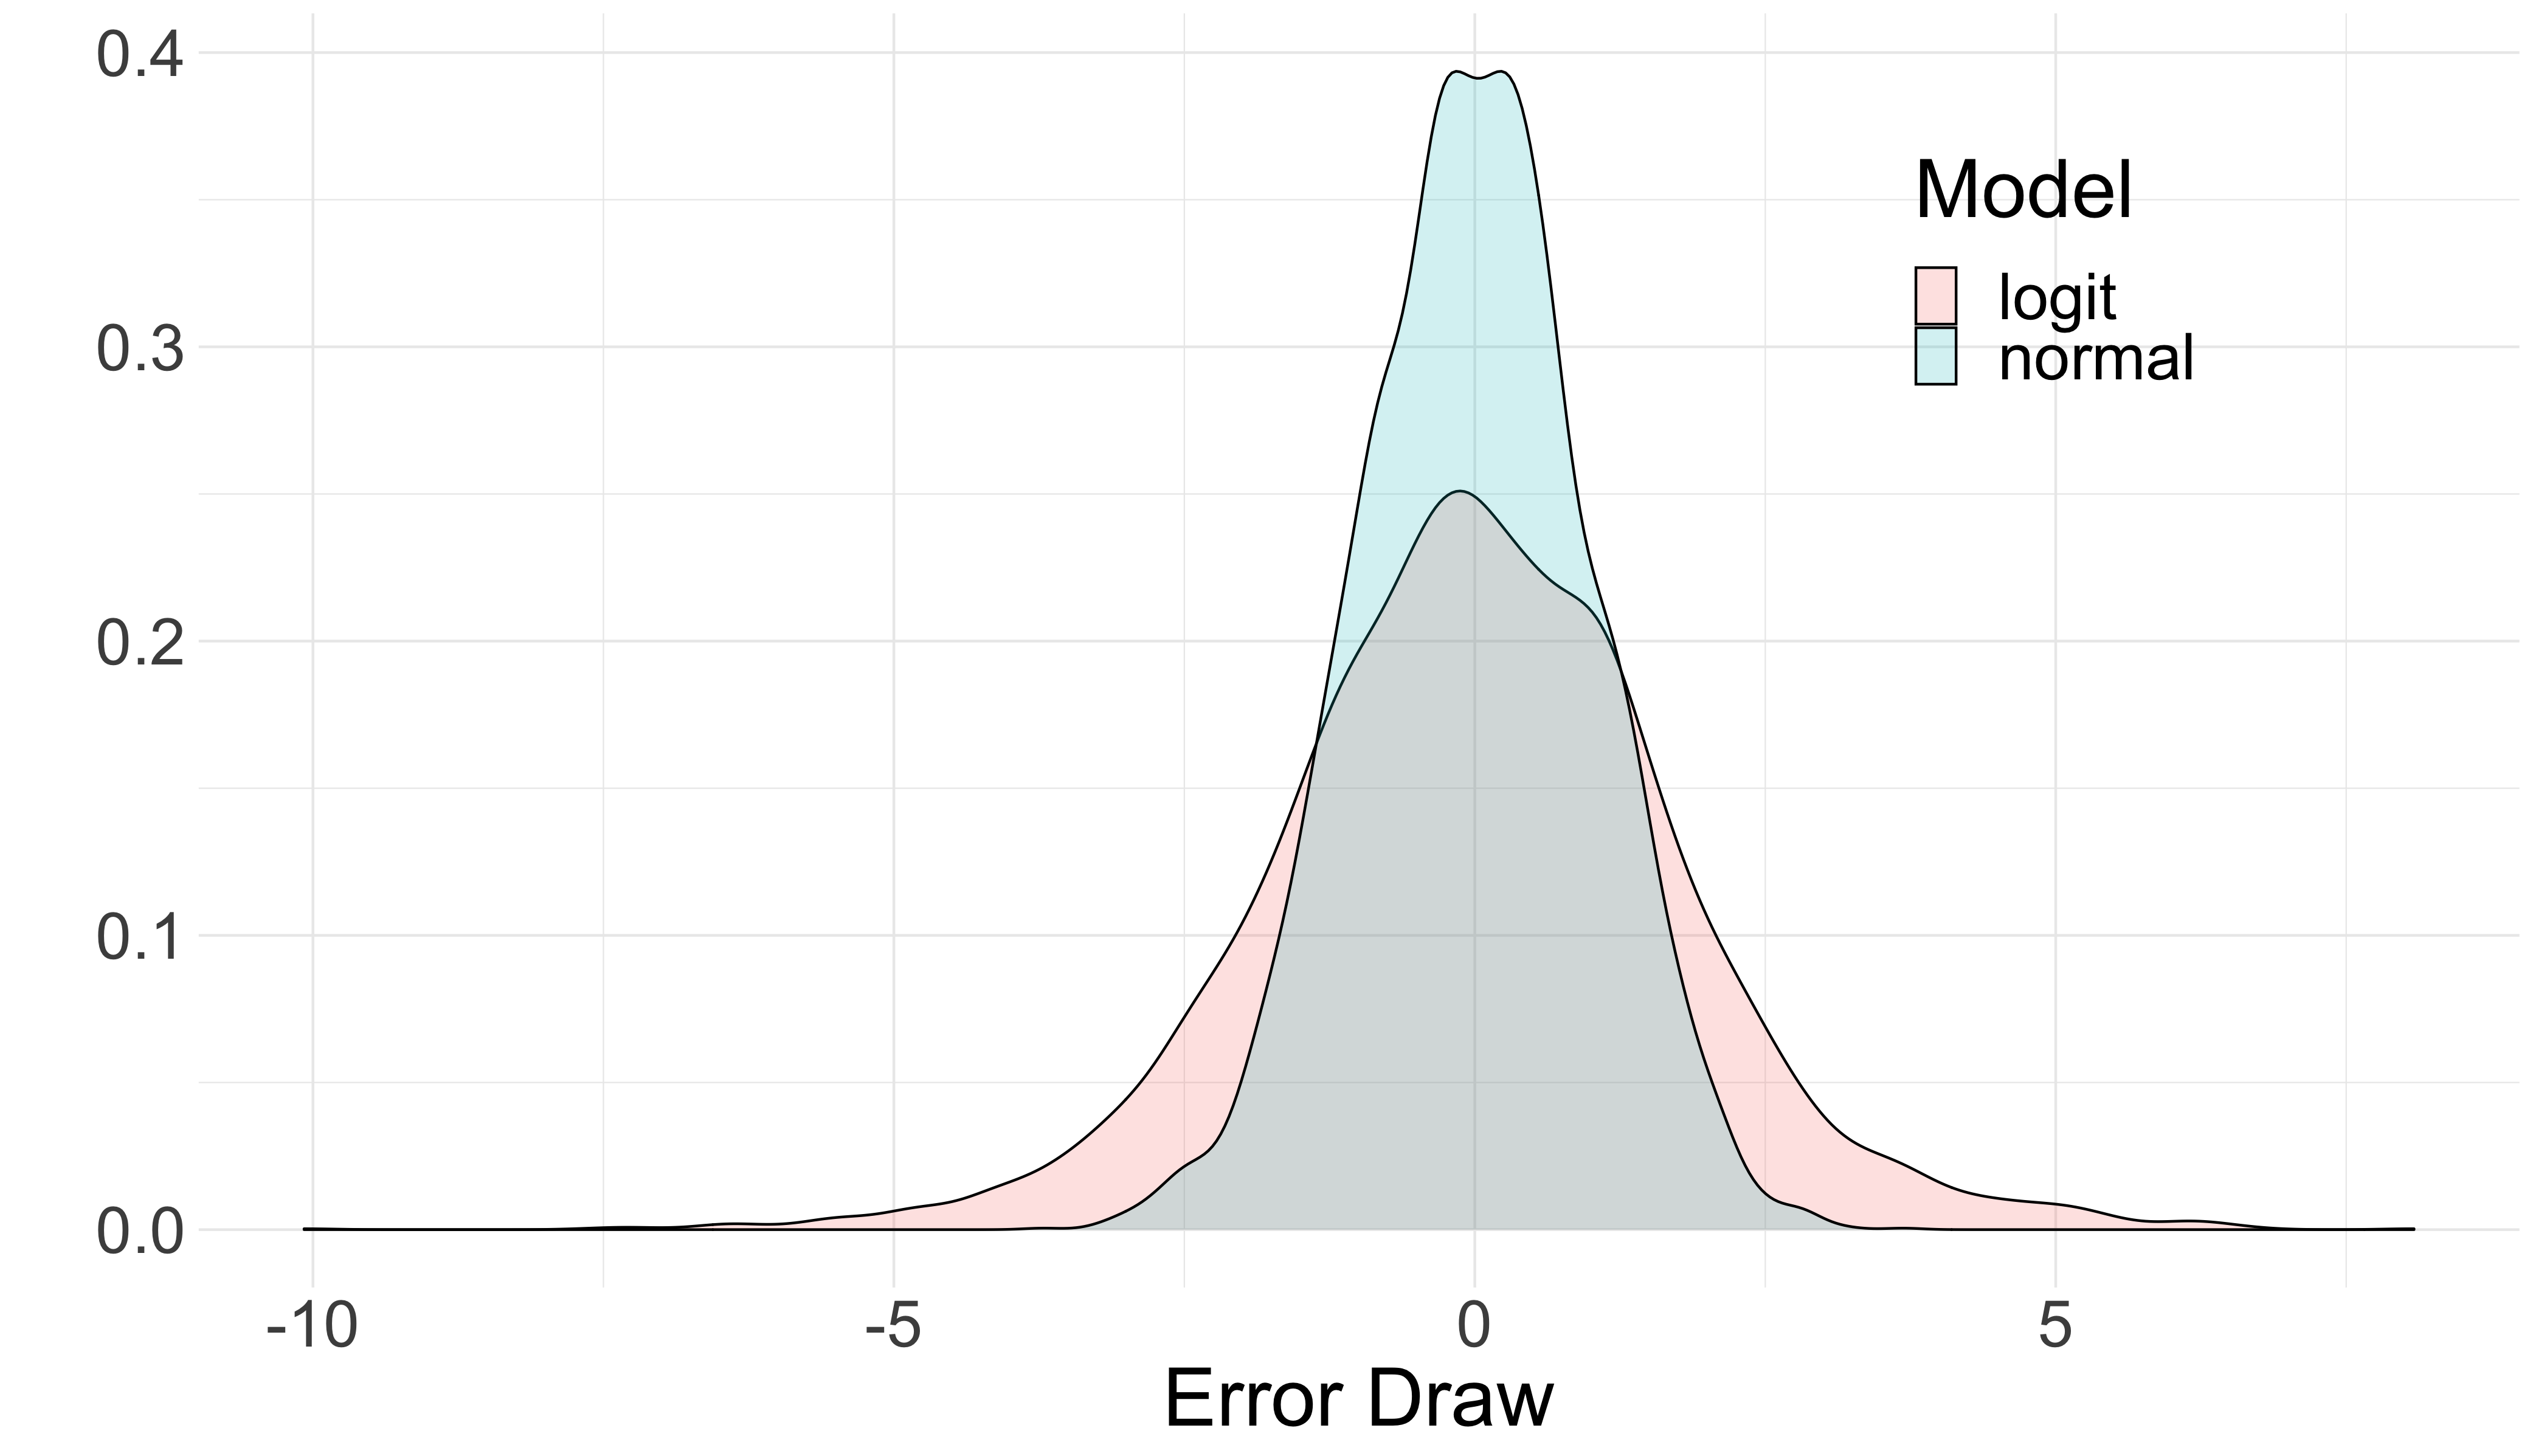
\includegraphics[width=\linewidth]{images/logit_v_normal.png}
    \end{center}
  \end{column}
\end{columns}
  \end{frame}

\begin{frame}{Comparing with Logit}
  \begin{columns}[T] % align columns
    \begin{column}{.35\textwidth}
      \begin{wideitemize}
      \item Consider now the same homeowner problem, but estimated with logit
      \item These coefficients are harder to interpret -- we can
        instead consider the average derivative:
        \begin{align*}
          &n^{-1}\sum_{i} \frac{\partial E(Y|X)}{\partial X} =\\
          &n^{-1}\sum_{i} \frac{\exp(X_{i}\beta)}{1+\exp(X_{i}\beta)}\frac{\beta}{1+\exp(X_{i}\beta)}
        \end{align*}
        \item Avg. deriv is comparable but not identical
      \end{wideitemize}
    \end{column}%
  \hfill%
  \begin{column}{.65\textwidth}
    \begin{center}
    \begin{tabular}{lrrr}
      term  &      logit est. & linear est. & avg. deriv. \\
      \midrule
      constant &      -2.14      &        0.0242 & -0.392 \\
      age      &         0.0903  &          0.022& 0.0166\\
      age$^{2}$ &          -0.0006&         -0.0002 & -0.0001\\
      income/10k     &       0.0716       &     0.0069 & 0.0131  
    \end{tabular}
  \end{center}
  \end{column}
\end{columns}
\end{frame}

\begin{frame}
  \begin{center}
    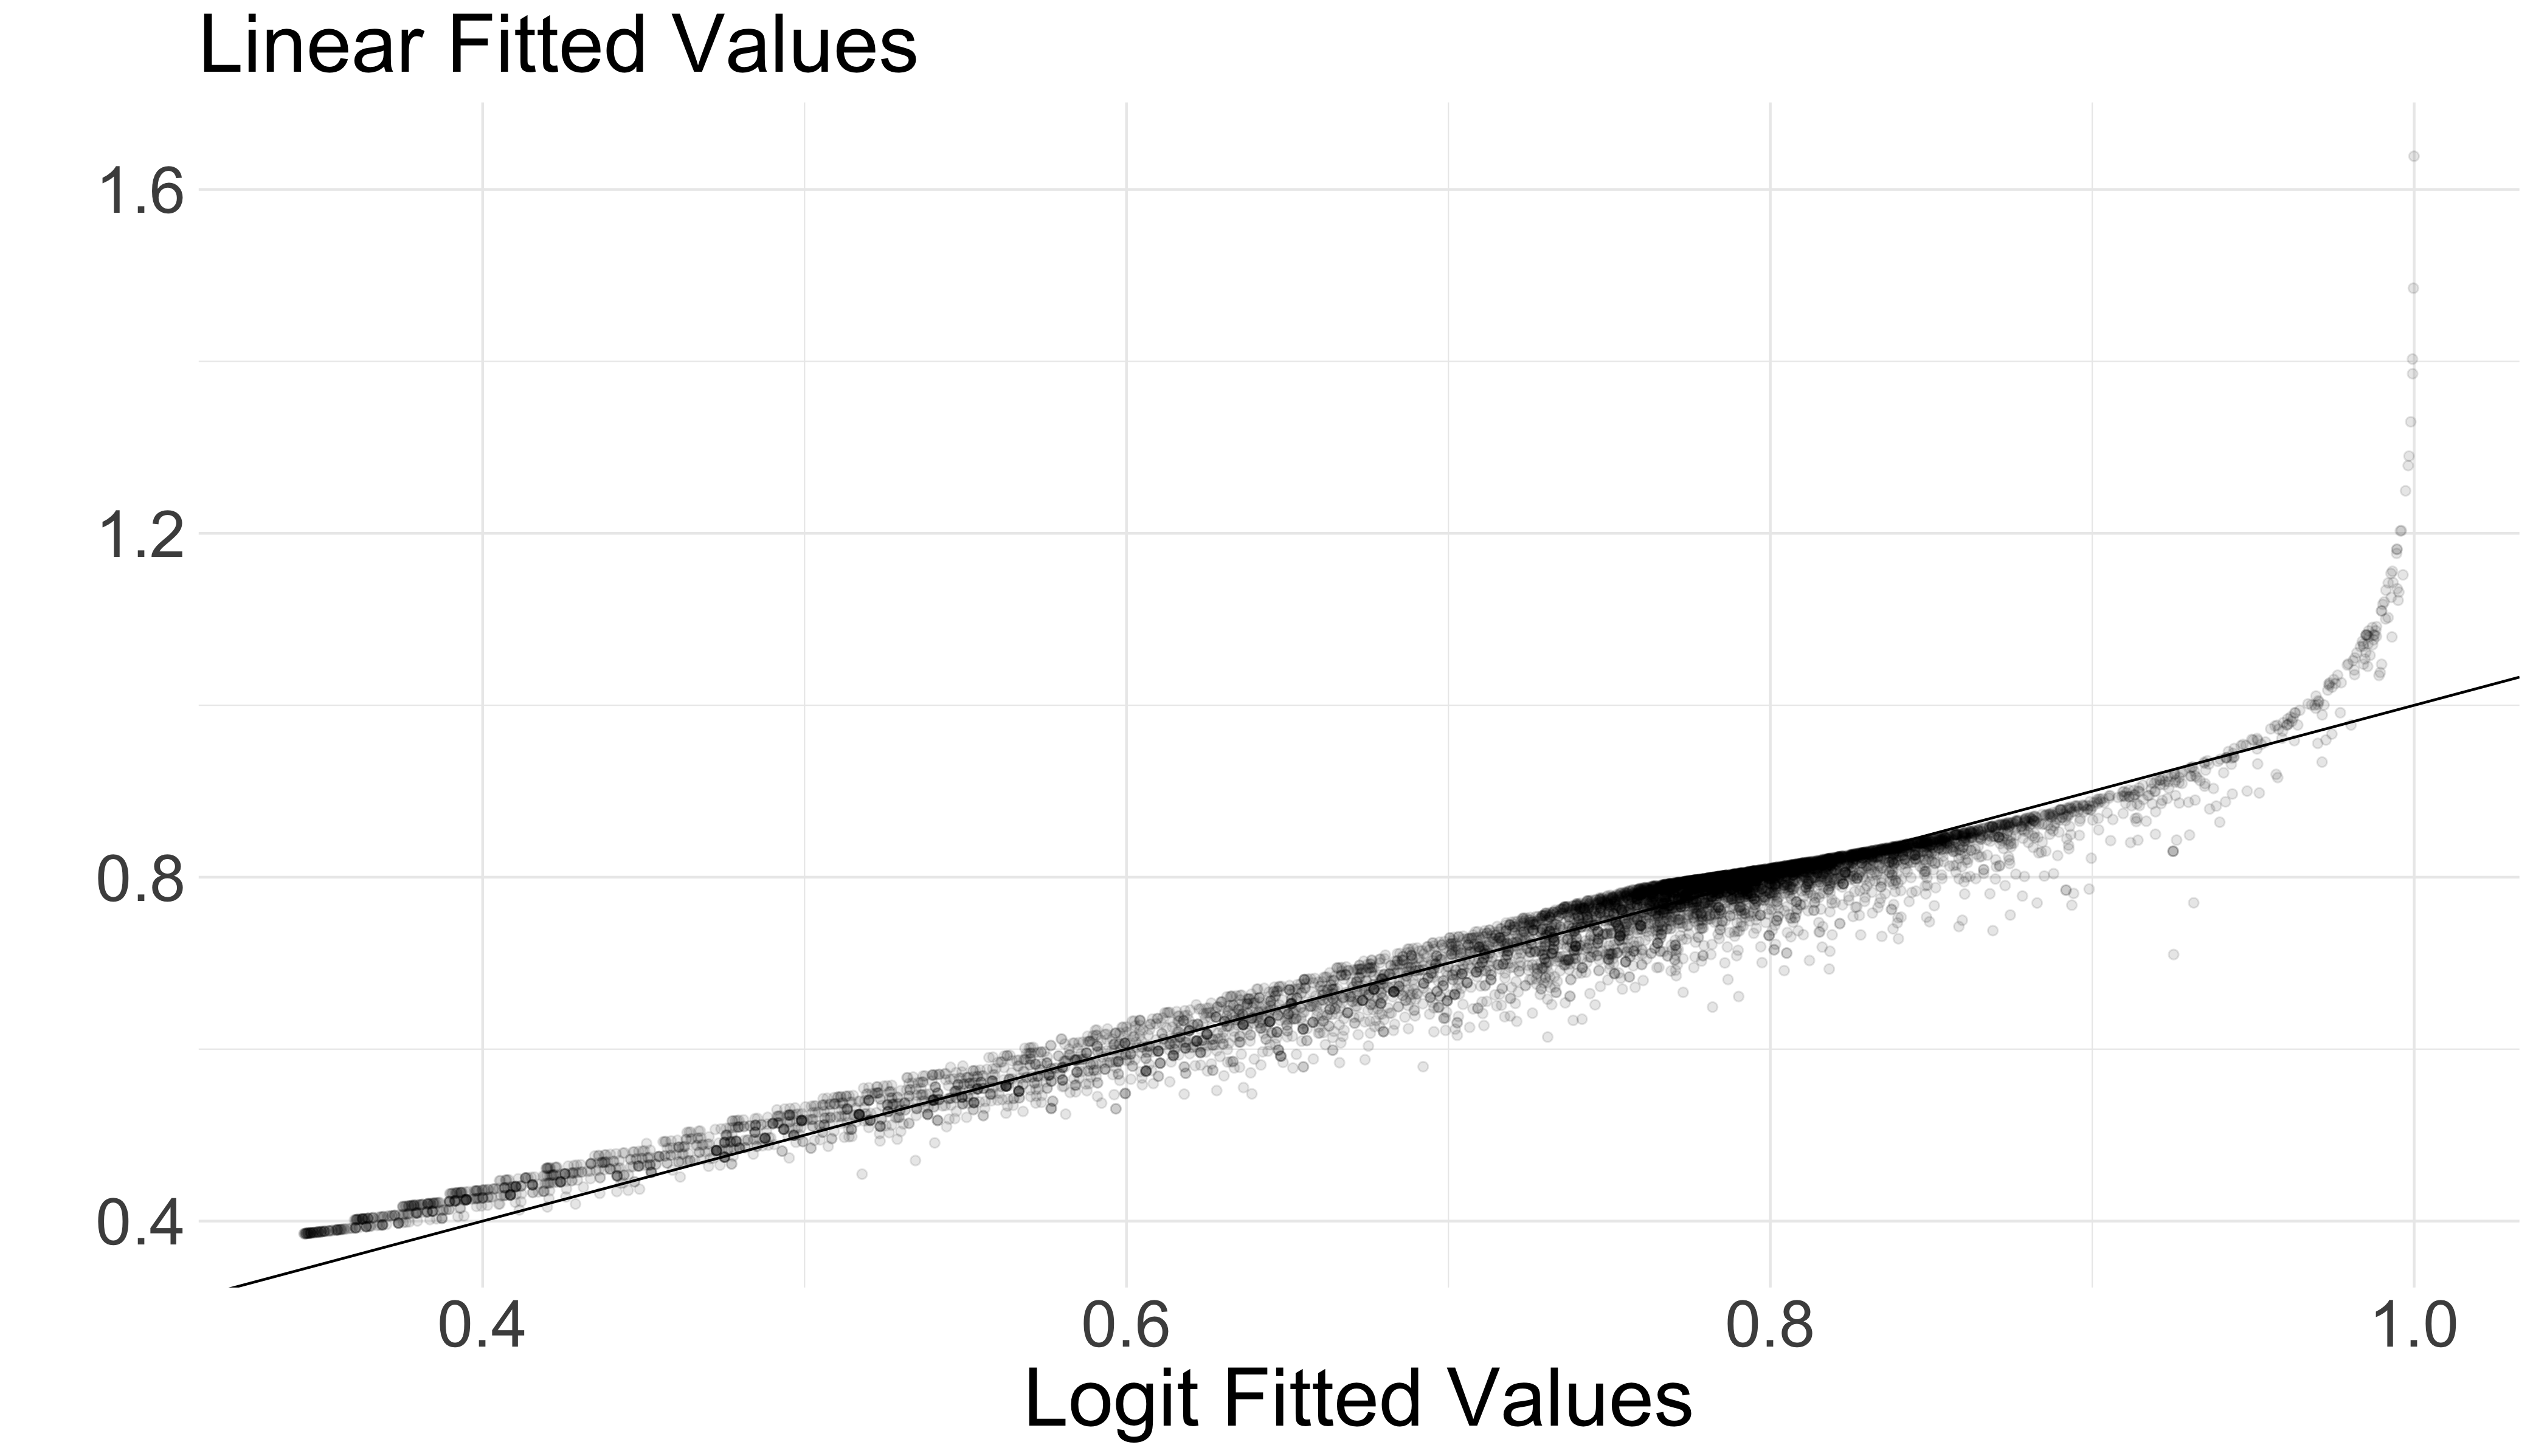
\includegraphics[width=0.8\linewidth]{images/linear_v_logit_scatter.png}
  \end{center}
\end{frame}
  
\begin{frame}{Aside: Generalized Linear Models}
  \begin{wideitemize}
    \item  Important aside: Generalized Linear Models (GLM)
      \begin{itemize}
      \item General setting considering errors that are non-normal
        (and may have restricted support)
      \item Very common terminology in non-economics settings
      \end{itemize}
    \item Key pieces with a linear model $X_{i}\beta$:
      \begin{enumerate}
      \item Link function $g$  such that $E(Y|X) = g^{-1}(X_{i}\beta)$
      \item Error distribution drawn from exponential family (includes normals, binomial, Poisson)
      \end{enumerate}
    \item Some simple examples:
      \begin{itemize}
      \item Logit (we just did this), with a link function $log\left(\frac{X_{i}\beta}{1-X_{i}\beta}\right)$
      \item Normal (we just did this), with an identity link function
      \end{itemize}
    \item In essence, we can enforce a linear functional form to the
      \emph{mean}, and allow the error distribution to fit the form of
      the data
      \begin{itemize}
      \item Important underused case: Poisson regression for
        non-negative numbers
      \item Key point: even if model is ``wrong'', can construct
        robust s.e. that are robust to the misspecification
      \end{itemize}
  \end{wideitemize}
  \end{frame}

  \begin{frame}{Aside: GLM + Poisson Regression with Counts}
    \begin{wideitemize}
    \item Consider $Y \geq 0$. We are almost always interested in the
      estimand of $dE(Y | X) / dX$. If we estimate this with simple linear regression, what are potential issues?
      \begin{itemize}
      \item Error term will be highly right-skewed $\rightarrow$
        Skewness leads to outliers that are super influential with
        OLS! (recall quantile reg)
      \item Likely heteroskedasticity $\rightarrow$ Poor performance
        in finite samples of point estimates and CI (especially given
        skeweness)
      \end{itemize}
    \item What are solutions people use? $\log(Y)$ What are issues here?
      \begin{itemize}
      \item Interpretation of parameters
      \item What if $Y = 0?$
      \end{itemize}
    \item What about $\log(1+Y)$?
      \begin{itemize}
      \item Solves the second problem, but makes the first problem even worse!
      \item Many people use this... (guilty)
      \end{itemize}
    \end{wideitemize}
  \end{frame}


  \begin{frame}{Aside: GLM + Poisson Regression with Counts}
    \begin{wideitemize}
    \item So what's the alternative? Poisson regression
      \begin{itemize}
      \item Key to this model is estimating $\log(E(Y|X)) = X\beta$,
        rather than $E(\log(Y)|X)$. You get a simple semi-elasticity
        measure for the parameters, and $Y$ can be zero.
      \end{itemize}
    \item What are the typical concerns?
      \begin{enumerate}
      \item       If $Y | X$ is truly distributed
      Poisson, conditional on $X$, then $Var(Y|X) = E(Y|X)$ which is a
      restrictive model assumption (just comes from the Poisson
      distribution's features)
      \begin{itemize}
      \item However, it's not relevant for the parameter estimates of
        $\beta$. The estimates are still consistent.
      \item Robust standard errors (using sandwich covariance
        estimators) will give correct coverage as well
      \end{itemize}
    \item Fixed effects in non-linear models?
      \begin{itemize}
      \item Typical concern is that in non-linear models, fixed
        effects that are not consistently estimated with bias estimate
        of main parameters (unlike in OLS)
      \item Turns out not to be an issue in Poisson, as fixed effects
        can be concentrated out (see PPMLHDFE in Stata and glmhdfe in
        R)
      \end{itemize}
    \item Can even use instrumental variables! (See Mullahy (1999) and
      Windmeijer and Santos Silva (1997))
    \end{enumerate}
  \item See Cohn, Liu and Wardlaw (2021) for a nice discussion in finance settings
    \end{wideitemize}
  \end{frame}


  
  % $
  \begin{frame}{How do we estimate these problems?}
    \begin{wideitemize}
    \item     How do we estimate these types of problems? Consider the likelihood function for logit:
    \begin{align*}
      Pr(Y_{i} = 1 | X_{i} ) &= \frac{\exp(X_{i}\beta)}{1+\exp(X_{i}\beta)}\\
      l(\beta|\mathbf{Y}, \mathbf{X}) &= \Pi_{i=1}^{n} Pr(Y_{i} = 1 | X_{i} )^{Y_{i}}(1-Pr(Y_{i} = 1 | X_{i} )^{1-Y_{i}}\\
      L(\beta|\mathbf{Y}, \mathbf{X}) &= \sum_{i=1}^{n} Y_{i}\log(Pr(Y_{i} = 1 | X_{i} ))\\
                             &+  (1-Y_{i})\log(1-Pr(Y_{i} = 1 | X_{i} ))
    \end{align*}
  \item Rule of thumb: the likelihood is the joint probability of the data
    \begin{itemize}
    \item We are exploiting the independent nature of the data
    \item Joint probability of two independent values is the product
      of their marginals
    \end{itemize}
  \item Recall that we can take the log of the likelihood when
    considering extremes of the function because any maximum will be
    identical irrespective of monotone transformations
  \end{wideitemize}
  \end{frame}

  \begin{frame}{Plug in Logit to the ML}
    \begin{wideitemize}
      
    \item    With some simple rewriting:
    \begin{align*}
      L(\beta|\mathbf{Y}, \mathbf{X}) &= \sum_{i=1}^{n} Y_{i}\log(\frac{\exp(X_{i}\beta)}{1+\exp(X_{i}\beta)} +  (1-Y_{i})\log(\frac{1}{1+\exp(X_{i}\beta)})\\
      &= \sum_{i=1}^{n} Y_{i}X_{i}\beta - Y_{i}\log(1+\exp(X_{i}\beta)) +  (1-Y_{i})\log(1+\exp(X_{i}\beta)))\\
      &= \sum_{i=1}^{n} Y_{i}X_{i}\beta - \log(1+\exp(X_{i}\beta))
    \end{align*}
    \item Great, so how would one estimate this? We have a likelihood, we want to maximize it!

    \item  Take derivatives and find the maximum!
      \begin{itemize}
      \item Finally that calculus is paying off!
      \end{itemize}

    \item Good news and bad news... 
    \end{wideitemize}
  \end{frame}

  \begin{frame}{The bad news and the good news}
    \begin{align*}
      L(\beta|\mathbf{Y}, \mathbf{X}) &= \sum_{i=1}^{n} Y_{i}X_{i}\beta - \log(1+\exp(X_{i}\beta))
    \end{align*}
    \begin{wideitemize}
    \item    There's no analytic solution for this $\beta$. Unlike with OLS, we
    can't get a closed-form solution for our estimate -- this is true
    of most estimators. In fact, this is a well-behaved problem,
    relative to most.
    \begin{itemize}
    \item Well-behaved because it's globally concave and has easily
      calculated first and second derivative
      
    \end{itemize}
  \item     So,  What's the good news? We have computers!
    \end{wideitemize}

  \end{frame}

  \begin{frame}{The bad news and the good news}
    \begin{align*}
      \frac{\partial L(\beta)}{\partial \beta} =  \sum_{i=1}^{n} X_{i}(Y_{i} - \frac{\exp(X_{i}\beta)}{1+\exp(X_{i}\beta)})
    \end{align*}
    \begin{wideitemize}
    \item While there is not an analytic solution, if there is a
      maximum where $\hat{\beta}$ satisfies
      $\frac{\partial L(\hat{\beta})}{\partial \beta} = 0$, then there
      are sets of conditions such that
      \begin{itemize}
      \item $\lim_{n\to\infty}\Pr(||\hat{\beta}_{n} - \beta_{0}|| > \epsilon) = 0$ (weak consistency)
      \item $\lim_{n\to\infty} \sqrt{n} (\hat{\beta}_{n} - \beta_{0}) \rightarrow^{d} \mathcal{N}\left(0, -E\left[\frac{\partial^{2}}{\partial\beta \beta'}L(\beta_{0})\right]\right)$ (asymptotic normality)
      \end{itemize}
    \item The challenge is that the conditions for when this is
      satisfied vary from problem to problem
    \item Most general results in this put high-level assumptions on
      the problem, and then the conditions need to be checked
    \end{wideitemize}
    
  \end{frame}


  \begin{frame}{The bad news and the good news}
    \begin{align*}
      \frac{\partial L(\beta)}{\partial \beta} =  \sum_{i=1}^{n} X_{i}(Y_{i} - \frac{\exp(X_{i}\beta)}{1+\exp(X_{i}\beta)})
    \end{align*}
    \begin{wideitemize}
    \item While there is not an analytic solution, if there is a
      maximum where $\hat{\beta}$ satisfies
      $\frac{\partial L(\hat{\beta})}{\partial \beta} = 0$, then there
      are sets of conditions such that
      \begin{itemize}
      \item $\lim_{n\to\infty}\Pr(||\hat{\beta}_{n} - \beta_{0}|| > \epsilon) = 0$ (weak consistency)
      \item $\lim_{n\to\infty} \sqrt{n} (\hat{\beta}_{n} - \beta_{0}) \rightarrow^{d} \mathcal{N}\left(0, -E\left[\frac{\partial^{2}}{\partial\beta \beta'}L(\beta_{0})\right]\right)$ (asymptotic normality)
      \end{itemize}
    \item The conditions for when this is satisfied vary from problem
      to problem
    \item Most general results in this put high-level assumptions on
      the problem, and then the conditions need to be checked for a particular problem
      \begin{itemize}
      \item These general types of problems are classified into $M$-estimation
        and $Z$-estimation
      \item $M$-estimation is a general problem where $\beta_{0} = \arg\max_{\beta} E(m(\beta))$
      \item $Z$-estimation $\subset$ $M$-estimation focused on
        exploiting features of the derivative of $m(\beta)$
      \end{itemize}
    \end{wideitemize}
  \end{frame}


  \begin{frame}{How to compute - Newton-Raphson}
    \begin{wideitemize}
    \item In our applications, very well-defined solutions. We'll
      instead focus on the actual computation of these maxima
    \item There are many numerical optimization methods. I'll outline
      info on the few I know, but this is in no way exhaustive
      \begin{itemize}
      \item This draws from my own graduate school notes!
      \end{itemize}
    \item A common simple method is Newton-Raphson

    \end{wideitemize}
  \end{frame}

  \begin{frame}{Newton-Raphson Computation of MLE}
    \begin{wideitemize}
    \item Let $Q(\theta) = -L(\theta)$ (denote with $\theta$ to
      highlight that this is a general problem)
    \item Idea is to take some arbitrary objective function and fit a
      local quadratic based on derivatives
      \begin{itemize}
      \item Find the minimum based on this quadratic
      \item Take that minimizer and repeat
      \end{itemize}
    \item Specifically, let
      $$ \theta_{k+1} = \theta_{k} - \left[\frac{\partial^{2}Q(\theta_{k})}{\partial\theta \partial \theta'}\right]^{-1}\frac{\partial Q}{\partial \theta}(\theta_{k})$$
    \item In our Logit application, we already know the first derivative -- calculating the second derivative is straightforward. Hence, we can solve for $\theta$
      \begin{itemize}
      \item We benefit from a convex problem and an easily defined second derivative
      \end{itemize}
    \end{wideitemize}
  \end{frame}

  \begin{frame}{More general methods}
    \begin{wideitemize}
    \item What if we don't know our second derivative? (or it is onerous to
    calculate)
    \item Then we can reframe to the problem in two pieces.  Let $A_{k}$ be
    any positive definite matrix. Consider the following iterated estimation:
    $$ \theta_{k+1} = \theta_{k} - \lambda_{k}A_{k}\frac{\partial Q}{\partial\theta}(\theta_{k})$$

  \item    This nests Newton-Raphson:
    \begin{itemize}
    \item $\lambda_{k} = 1$
    \item $A_{k} = \left[\frac{\partial^{2}}{\partial\theta \theta}L(\theta_{k})\right]^{-1}$
    \end{itemize}

  \item    Intuitively, there are two pieces:
    \begin{itemize}
    \item  a steplength (defined by $\lambda_{k}$)
    \item a direction
      $d_{k} = A_{k}\frac{\partial Q}{\partial\theta}(\theta_{k})$
      (controlled by $A_{k}$, which select a direction of the
      gradient)
      \begin{itemize}
      \item A convenient rescaling is $\tilde{d}_{k} = d_{k} / (1 + \sqrt{d_{k}'d_{k}}$ to ensure $|\tilde{d}_{k}| < 1$
      \end{itemize}
    \end{itemize}
    \end{wideitemize}
  \end{frame}
  \begin{frame}{Simple version of algorithm}
    \begin{wideitemize}
    \item We can choose the direction, then choose how far we want to go
      $$\lambda_{k} = \arg\min_{\lambda}Q(\theta_{k} + \lambda \tilde{d}_{k})   $$
    \item Simplest version verison of this is $A_{k} = I_{k}$
      (identity matrix) -- just go in the direction of steepest
      descent
    \item How does one calculate $\lambda_{k}$ in these settings? If
      $\theta$ is scalar, it's feasible (but inefficient) to calculate
      using a simple grid search 
    \item In high-dimensions, too slow (and our next algorithm needs
      optimal choice to converge)
    \end{wideitemize}
  \end{frame}


  \begin{frame}{Two line search algorithms - Newton's Method}
    \begin{wideitemize}
    \item Given a $d$, recall we need a $\lambda$. Redefine $\lambda^{*} = \arg\min_{\lambda} Q(\lambda)$
    \item The simplest method is Newton's method (which finds the root
      of a function (we want the root of the derivative)
    \item Begin with an initial guess for $\lambda_{0}$. Then,
      $$\lambda_{k+1} = \lambda_{k} - \frac{Q'(\lambda_{k})}{Q''(\lambda_{k})}$$
      %$
      Repeat till $|\lambda_{k+1}-\lambda_{k}|$ is small
      (e.g. convergence)
    \item Issue with this approach is you need a second derivative
    \end{wideitemize}
  \end{frame}

  \begin{frame}{Two line search algorithms - Golden Search}
    \begin{wideitemize}
    \item Start with two points you know for certain contain the minimum (need unimodality)
      \begin{itemize}
      \item E.g. $\lambda_{l} = 0, \lambda_{h} =
        1$ [Picking an abritraily large $\lambda_{h}$ is fine -- there
        are ways to check this]
      \end{itemize}
    \item Two points on the line segment between: $\lambda_{m1} = \lambda_{l} + 0.392 \times (\lambda_{h} - \lambda_{l})$ and $\lambda_{m2} = \lambda_{l} + 0.618 \times (\lambda_{h} - \lambda_{l})$
    \item Now, given the four points, can check two conditions:
      \begin{itemize}
      \item $Q(\lambda_{m2}) > Q(\lambda_{m1})$: you know that the minimizing value of  $\lambda $ in [$\lambda_{l}$, $\lambda_{m2}$]. Update your values:  $\lambda_{l}' = \lambda_{l}$, $\lambda_{h}' = \lambda_{m2}$, $\lambda_{m2}' = \lambda_{m1}$, $\lambda_{m1}' =  \lambda_{l}' + (\lambda'_{h} - \lambda'_{m2}$
      \item $Q(\lambda_{m2}) < Q(\lambda_{m1})$: you know that the minimizing value of  $\lambda $ in [$\lambda_{m1}$, $\lambda_{h}$]. Update your values:  $\lambda_{h}' = \lambda_{h}$, $\lambda_{l}' = \lambda_{m1}$, $\lambda_{m1}' = \lambda_{m2}$, $\lambda_{m2}' =  \lambda_{h}' - (\lambda'_{m1} - \lambda'_{l}$
      \end{itemize}
    \item Update until you find the optimal $\lambda$
    \end{wideitemize}
  \end{frame}

  \begin{frame}{Davidson-Fletcher-Powell}
    \begin{wideitemize}
    \item DFP is more elaborate, and requires all these pieces
      \begin{itemize}
      \item Commonly used, although not the fastest algorithm out there now
      \end{itemize}
    \item Its strongest feature is that it is efficient and can work
      without calculating a second derivative
    \item Initiate with any positive definite matrix $A$
      (e.g. identity matrix)
    \item Steps (repeat till convergence):
      \begin{enumerate}
      \item Calculate direction $\tilde{d}_{k}$
      \item Calculate optimal step length $\lambda_{k}$
      \item Calculate the actual step
        $p_{k} = \lambda_{k}\tilde{d}_{k}$ and the new parameter
        $\theta_{k+1} = \theta_{k}+ p_{k}$
      \item Calculate the change in the derivative $q_{k}$ from
        $\theta_{k}$ to $\theta_{k+1}$
      \item Update
        $$A_{k+1} = A_{k} + \frac{p_{k}p_{k}'}{p_{k}'q_{k+1}} - \frac{A_{k}q_{k+1}q_{k+1}'A_{k}}{q_{k+1}'A_{k}q_{k+1}}$$
      \end{enumerate}
    \end{wideitemize}
  \end{frame}
\end{document}